\chapter{Recherche d'information}
\section{Introduction}
La recherche d'information est un domaine étendu et ancien qui trouve ses racines au début des années 1950, peu après l'invention de l'ordinateur \citep{approche-semantique}. Plus précisément, elle date des années 1940 dès la naissance de l'ordinateur. Dans les années 1960 et 1970, la RI commence les expérimentations plus larges alors qu'au départ elle s'est concentré sur des applications des bibliothèques. Et puis l'intégration de l'IA dans la RI a partir des années 1980 ainsi que la naissance d'internet en 1990 propulse la RI et met en scène beaucoup d'applications. \citep{salton1989automatique}

La RI suscite donc un grand intérêt parmi les chercheurs, devenant de plus en plus attrayante avec l'avènement de machines puissantes et performantes en matière de stockage, faciles à utiliser et fiables \citep{evaluation-of-ir-system}. La recherche d'information est désormais une tâche récurrente pour les utilisateurs, que ce soit sur smartphones, ordinateurs, etc., car elle répond à leurs besoins quotidiens \citep{thesaurus-ir-web}. Ce domaine traite des données non structurées, principalement des données textuelles comme le langage naturel \citep{modern-ir}.
Citons quelques définitions de la Recherche d'Information:

\begin{definition}
    Selon Gérard Salton, père de la Recherche d'Information, la RI consiste a structurer, analyser, organiser, stocker, et rechercher de l'information. \citep{thesaurus-ir-web}
\end{definition}

\begin{definition}
    Un activité de délivrer un ensemble des documents a l'utilisateur en fonction de son besoin d'information (\cite{thesaurus-ir-web}).
\end{definition}

\begin{definition}
    C'est la Stockage, Gestion, Traitement, récupération des informations, documents ou site web pour satisfaire un besoin informationnel de l'utilisateur \citep{vsm-for-arabic-language}.
\end{definition}

\begin{definition}
    La RI est un ensemble d'une base de documents et une phase de processus de recherche avec des méthodes, techniques permettant a l'utilisateur de récupérer un ou plusieurs documents \citep{ri-sur-le-web}.
\end{definition}

\begin{definition}[Système de Recherche d'Information]
    On appelle SRI ou moteur de recherche, un ensemble de programmes informatiques, qui met en œuvre des techniques et moyens pour trouver les documents pertinents afin de satisfaire le besoin d'information de l'utilisateur \citep{approche-semantique}.
\end{definition}

Voici un courte historique de la recherche d'information jusqu'au 1998 qui est l'arrivé de Google, illustré dans la Figure~\ref{fig:ir-history}.

\begin{figure}[htbp]
    \begin{center}
        \fbox{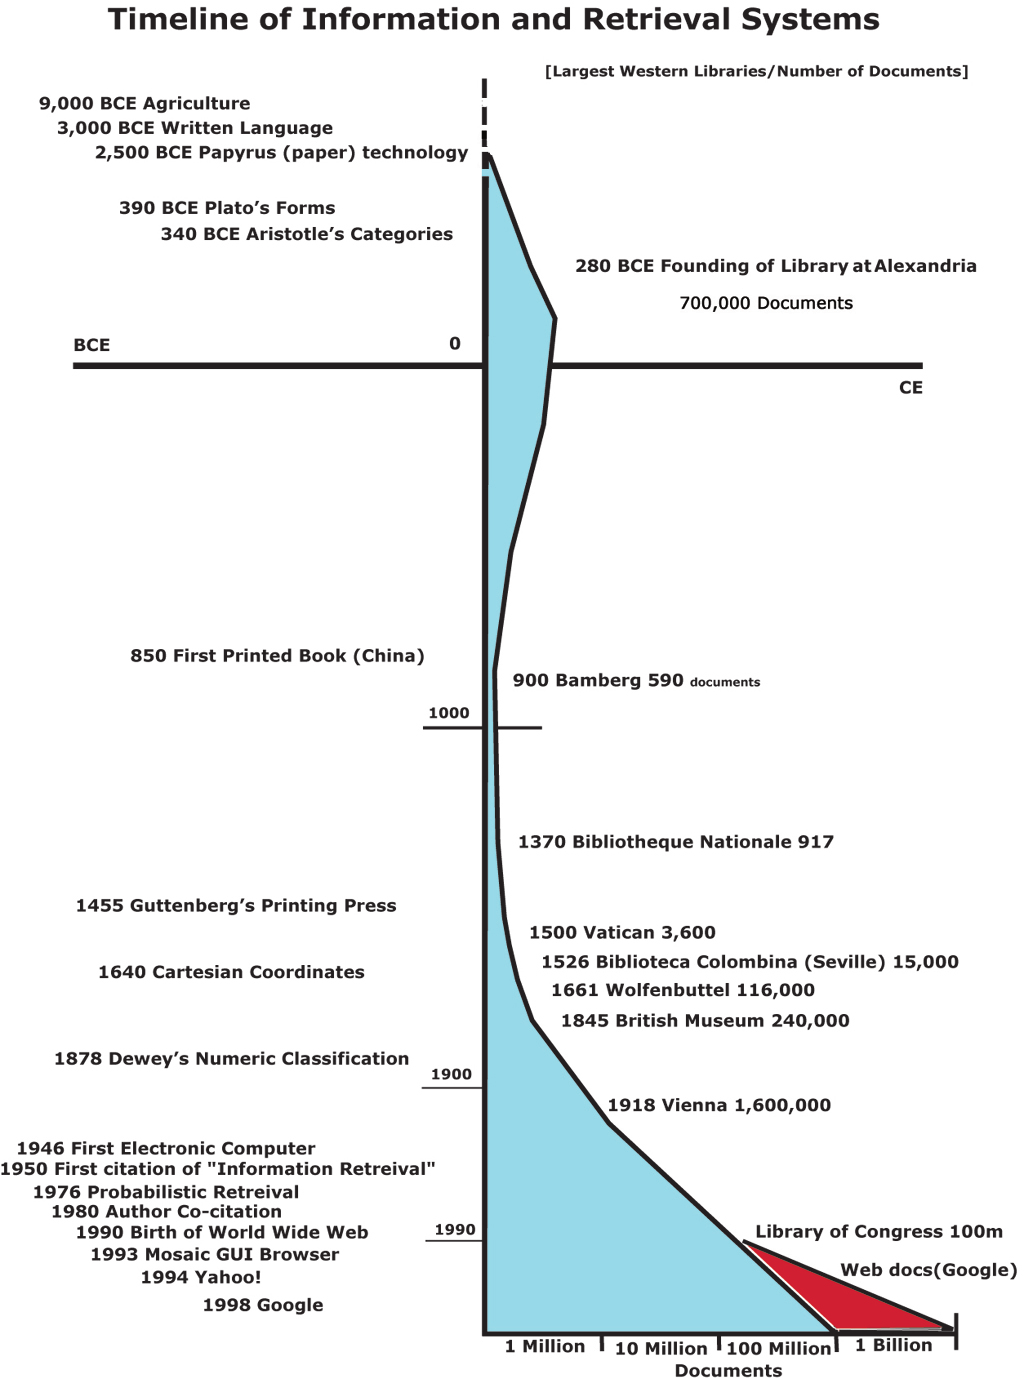
\includegraphics[width=15cm, angle=0]{Figures/ir-history.png}}
    \end{center}
    \caption{Historique de la recherche d'information \citep{ir-course}}
    \label{fig:ir-history}
\end{figure}

Le principe de base de la recherche d'information est illustré dans la Figure~\ref{fig:processus-ri}.

\begin{figure}[htbp]
    \begin{center}
        \fbox{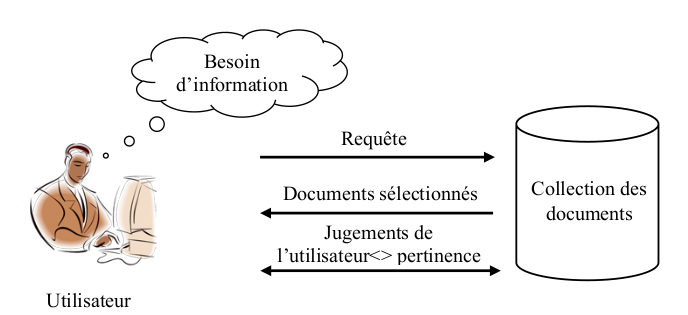
\includegraphics[width=15cm, angle=0]{Figures/processus-ri-simple.png}}
    \end{center}
    \caption{Processus de base de la RI \citep{amelioration-ri-approche-semantique}}
    \label{fig:processus-ri}
\end{figure}

\section{Pourquoi rechercher une information ?}
Lorsqu'un utilisateur a un besoin informationnel (Besoin d'information) la RI est nécessaire pour satisfaire ce besoin. D'où l'initiation de sa Recherche d'information. C'est le besoin d'information de l'utilisateur qui déclenche alors le processus de RI qu'on va voir dans la section suivante.

Le défi de la recherche d'informations est de satisfaire le mieux la demande de l'utilisateur en retournant un ensemble des documents correspondant a ses demandes parmi un grand volume de documents \citep{amelioration-ri-approche-semantique}.

\section{C'est quoi une information ?}
Une information est issu lorsqu'on donne un sens a un données. Un donnée est donc un unité élémentaire d'information, un octets constitué de bits c'est à dire des 0 et des 1. Un donnée est une représentation a laquelle une signification peur être rattaché, peut être quantitative ou qualitative et n'a pas de chance elle-même.

Une information est donc une collection des données pour donner une forme a une message que ce soit imagée, écrite ou orale pour réduire l’incertitude et transmettre quelque chose qui déclenche une action \citep{thesaurus-ir-web}, \citep{construction-memoire-organisationnel-benayache}.

Selon \citeauthor{j-velo:sys-user} \citep{j-velo:sys-user} une information est définie comme un fait, une réalité, qui augmente la connaissance des individus. Elle est constitué de \textit{données} et de \textit{sens} qui est attribué par un individu. Le sens dépend de l'individu qui reçoit la données.

\section{C'est quoi un document ?}
\citeauthor{thesaurus-ir-web} propose quelques définitions d'un document, on va citer deux parmi ceux qui sont cité \citep{thesaurus-ir-web}.

\begin{definition}
    Un document est généralement l'expression d'une pensée humaine.
\end{definition}

\begin{definition}
    Un document représente toute base de connaissance fixé matériellement, susceptible d'être utilisé pour la consultation, l'étude ou la preuve (imprimé, manuscrit, représentation graphique, \dots).
\end{definition}

\begin{definition}
    On appelle document toute unité qui peut constituer une réponse à une requête d'utilisateur. Un document peut être un texte, un morceau de texte, une page Web (HTML), une image, une bande vidéo, sons, etc \citep{salton1989automatique}.
\end{definition}

Un document composé de cinq éléments \citep{thesaurus-ir-web}:
\begin{itemize}
    \item \textbf{Support d'enregistrement}: papier, disque magnétique, CD/DVD-ROM, etc. C'est un support où le document est stocké.
    \item \textbf{Forme d'enregistrement}: papier, codage ascii, codage vidéos, etc. C'est la forme de document dans le support.
    \item \textbf{Support de restitution}: papier, écran d'ordinateur, haut-parleurs, etc.
    \item \textbf{Forme physique de restitution}: écran sur papier, signal audio ou vidéos, etc.
    \item \textbf{Forme sémantique de restitution}: représentation qui respecte une certaine structure ou forme selon laquelle elle soit intelligible par le l'utilisateur. Écriture, sons, images, animés, etc.
\end{itemize}

Par la suite de ce recherche, nous traitons des documents textuelles, non structurés.

\section{Classification des documents}
\subsection{Type de classification des documents}
Pour pouvoir récupérer les documents qui sont similaires, ainsi que pour faciliter le filtrage des résultats par l'utilisateur, il est important de classifier les documents.

La classification des documents est donc de grouper les documents similaire ensemble dans un classe. Cette opération se fait sur la collection des documents ou corpus. Il y a deux types de classification \citep*{modern-ir} tel que la classification \textit{local} et la classification \textit{global}:
\begin{itemize}
    \item \textbf{Classification global}: les documents sont groupés selon leur occurrences dans la collection.
    \item \textbf{Classification local}: les groupement des documents est affecté par le contexte défini par la requête et les documents local sélectionné. La classification varie selon la requête de l'utilisateur.
\end{itemize}

\subsection{Algorithmes de classification global}
Il y a beaucoup des algorithmes qui permet de classifier les documents textuels, dont certains se base sur l'algorithme du Machine Learning (ML) et de l'Intelligence Artificiel (AI). Voyons quelques algorithmes cité dans quelques revue scientifique des classifications des documents textuels \citep*{classification-text-documents,classification-text-documents-ml}.

Pour l'approche du machine learning, il y a des algorithmes qui se base sur l'apprentissage supervisé, l'apprentissage non supervisé et l'apprentissage par renforcement.

\begin{itemize}
    \item \textbf{K-Plus Proche Voisin ou K-Nearest Neighboor (KPP ou KNN)}: Est utilisé pour classifier des textes. L'approche définit \textit{K} classe pour classifier. C'est un approche non paramétric. Pour décider si $d_{i}$ appartient a la classe $C_{k}$, la similarité ou la dissimilarité pour tous les documents $d_{j}$ dans le donnés d’entraînement est déterminé.
    \item \textbf{Arbre de décision}: La décision est basé sur certains conditions, et utilise un arbre. Les règles de classification sont représentés a travers la chemin du racine au feuille. L'algorithme d'arbre de décision le plus connu est \textit{ID3} et ses successeurs tel que \textit{C4.5} et \textit{C5}. Cette approche a des avantages comme, simple a expliquer et a comprendre par des personnes non connaisseur du domaine, simple a mettre en place ainsi utile dans les analyses prédictives.
    \item \textbf{Naive Bayes Classifier}: Est un algorithme de machine learning, et généralement utilisé pour classifier les documents WEB, qui est un approche probabiliste. Permet de catégoriser des documents, des news, etc. Cette algorithme est efficace, et qui nécessite moins de données d’entraînement, ainsi le résultat est efficace.
    \item \textbf{Support Vector Machine}: Est une approche supervisé du ML. Le SVM Classifie les données dans différentes classe par la recherche du ligne qui sépare les données d'entrainement en classes, on l'appelle ligne d'hyperplan. Il y a deux catégories tel que le \textit{SVM} linéaire et le \textit{SVM} non linéaire. Cette approche est performant pour classifier les données d’entraînement ainsi corrige bien la classification pour les futures données.
    \item \textbf{D'autres algorithmes}: Il y a encore d'autres algorithmes pour classifier les documents mais on va pas rentrer dans les détails dans le cadre de ce mémoire.
\end{itemize}

\section{Besoin d'information}
\label{sec:besoin-information}
\begin{definition}
    C'est la besoin d'information qui déclenche la recherche d'information de l'utilisateur comme cité ci-dessus. C'est une sensation qui porterait un individu a s'engager dans une activité de recherche d'information (\cite{thesaurus-ir-web}).
\end{definition}

\begin{definition}
    C'est une abstraction mentale dont l'utilisateur a besoin pour répondre a une question ou demande particulière et qui est exprimé en langage naturel \citep{amelioration-ri-approche-semantique} (Reformulation nécessaire).
\end{definition}

C'est cette besoin d'information que l'utilisateur doit traduire pour obtenir une requête afin qu'un SRI puisse satisfaire ce besoin, on dit souvent des mots clés de recherche \citep{modern-ir}.

La besoin d'information se catégorisent en trois types selon \citeauthor{paradis:tel-00005009} \citep{paradis:tel-00005009} tel que:
\begin{itemize}
    \item[•] \textbf{Besoin vérificatif}: l'utilisateur recherche une donnée particulière, et savoir comment y accéder pour vérifier le texte avec des données qu'il possède déjà. En d'autre terme, l'utilisateur possède déjà les données ou la partie mais il a besoin de vérification. Le besoin ne change pas au cours de sa recherche, on dit que c'est \textit{stable}.
    \item[•] \textbf{Besoin thématique connu}: l'utilisateur cherche a éclaircir, revoir ou trouver des nouvelles informations concernant un sujet ou domaine connu. La besoin peut changer (\textit{stable}) ou non (\textit{variable}) au cours de sa recherche ainsi qu'il peut se raffiner. Le besoin peut s'exprimer de façon incomplète.
    \item[•] \textbf{Besoin thématique inconnu}: l'utilisateur cherche des nouveaux concepts ou relations hors des domaines ou sujet connus. La besoin est variable et toujours exprimé de façon incomplète.
\end{itemize}

Pour mieux élaborer ce processus, on va analyser dans la section suivante la processus général de la recherche d'information, la processus en U.

\section{Tâche de recherche de l'utilisateur}
Une tache de recherche c'est qu'un utilisateur doit faire pour satisfaire un besoin d'information \citep*{boubee-tricot-2010,ri-sur-le-web}.
Les taches se catégorisent suivant deux types, une tache fermé et une tache ouverte. Une tâche fermé est une tache dont l'utilisateur cherche une réponse exacte sur une requête donnée, tandis qu'une tache ouverte est une tâche dont l'utilisateur cherche une réponse acceptable. Après certains études cités dans \citep{ri-sur-le-web} et d'autres chercheurs, que la tache ouverte utilise d'avantage la navigation, tandis que la tache fermé privilégie les moteurs de recherche.

Il y a deux stratégies de recherche cité par \citeauthor{ir-on-web} \citep{ir-on-web} en utilisant des requêtes:
\begin{itemize}
    \item[•] \textbf{Bottom-up ou mixtes:} la recherche commence par une sphère étroite (précise) puis l’élargir de plus en plus. L'utilisateur fait une recherche de plus précise a une recherche plus générale.
    \item[•] \textbf{Top-down:} la recherche commence par une sphère large (générale) puis le rétrécir de plus en plus. L'utilisateur fait une recherche de plus générale a une recherche de plus en plus précise.
\end{itemize}

Selon \citeauthor{ri-sur-le-web} \citep{ri-sur-le-web}, il y a trois type de taches:
\begin{itemize}
    \item[•] \textbf{Tache factuelle} est une tâche généralement fermé
    \item[•] \textbf{Tache interprétative} est une tâche généralement ouverte
    \item[•] \textbf{Tache d'exploitation} est une tâche complètement ouverte
\end{itemize}

\subsection{Tache factuelle}
Une tache factuelle est catégorisé dans la tache fermé, on peut le considérer comme une tache fermé. Dans une tache factuelle, les utilisateurs formulent de requêtes dans un SRI ou moteur de recherche, et lisent les résumés de chaque document dans la page de résultat. Ils veulent trouver une réponse sur la page de résultat et privilégie le résumé qui contient les mots clés, et en cliquant juste pour confirmation. Dans cette tache les experts utilise plutôt la stratégie bottom-up tandis que les novices utilisent la stratégie bottom-up \citep{ri-sur-le-web}.

\subsection{Tache interprétative}
Une tache factuelle est catégorisé dans la tache ouverte, on peut le considérer comme une tache ouverte. Les utilisateurs commencent par le parcours des informations générales, puis affiner leurs recherche pour leurs besoins spécifiques. Ils privilégié la lecture de contenu des pages et la navigation, souvent une navigation interne a des pages web (via des liens internes) ou externes.

\subsection{Tache d'exploitation}
Une tache d'exploitation est une tache complètement ouverte. Les utilisateurs se concentrent plus sur la page de résultat pour trouver une résultat qui semble correspondre au besoin, puis cliquent et naviguent dans la page pour explorer. Ils veulent trouver de l'information basé sur les contenues de la page. Dans cette tache, les experts utilisent la stratégie top-down tandis que les novices utilisent la stratégie bottom-up \citep{ri-sur-le-web}.

\section{Modèle de recherche de l'utilisateur}
En général il y a deux approche de recherche d'information, dont l'approche classique qui est le Ad-hoc et et l'approche moderne qui est le Filtering (Filtre en français) \citep{modern-ir}.

\subsection{Ad-hoc: approche classique}
L'approche classique est l'approche la plus utilisée, d'où c'est une approche conventionnel de la Recherche de l'Information. Dans une approche classique, les documents sont resté relativement statique (Les documents sont préparés a l'avance). Puis arrivé ensuite la requête des utilisateurs pour trouver une réponses dans ces documents. En d'autre terme, les documents restent statique jusqu’à ce que la requête de l'utilisateur arrive.

\subsection{Filtering: approche moderne}
L'approche moderne consiste a mettre en place un profile complexe de l'utilisateur pour savoir quel documents ou informations pourra lui interrelié. Dans cette approche, les requêtes (préférences, type d'informations qui lui intéressent, \dots) de l'utilisateur restent statique jusqu’à ce qu'un nouveau document arrive dans le système, et que ce système décide si c'est pertinent par rapport au profil de l'utilisateur. Cette approche est souvent utilisé pour les news, marketing, \dots

\section{Facteur d'influence de la recherche d'information}
La recherche d'information de l'utilisateur est influencé par plusieurs facteurs, tel que l'expérience, facteur socio-culturel, et d'autres facteurs.
On peut citer d'après l'analyse de ces facteurs fait par \citeauthor{ri-sur-le-web} \citep{ri-sur-le-web} les facteurs ci-dessous:
\begin{itemize}
    \item \textbf{Expérience de l'utilisateur}: l'expertise du domaine implique la qualité de choix des mots clés a utiliser, la stratégie de recherche; l'expertise du système implique la connaissance de fonctionnement d'un SRI et la stratégie de la RI; expertise RI implique la capacité d'utiliser un SRI spécifique.
    \item \textbf{Tache de recherche}: influencé par le type de tache de l'utilisateur, qu'il recherche de réponse exacte (\textit{tache fermé}) ou recherche de réponse acceptable (\textit{tache ouverte}).
    \item \textbf{Facteur socio-culturel}: la contexte sociale et la culture est indissociable de la recherche d'information; le genre influence aussi la recherche, la stratégie de recherche utilisé par les femmes est différente de celle de l'homme, et la chance de réussite est différente; l'âge aussi a son influence, les jeunes et les personnes âgés ont différente façon de faire une recherche. Par exemple, les jeunes on tendance a consulter moins de pages et formuler des requête plus souvent que les âgées.
    \item \textbf{Connaissance de fonctionnement de SRI}: parfois les connaissances sont fausse par rapport aux capacités des moteurs de recherche. L'utilisateur estime qu'il sait utiliser un SRI alors qu'il n'exploite véritablement les capacités du SRI.
    \item \textbf{D'autres facteurs}: d'autres facteurs sont aussi détaillés dans la section 2.2.5, comme la limite de temps, caractéristiques individuelles. Un tableau de synthèse de ces facteurs est présenté dans la section 2.3.
\end{itemize}

Pour plus de détails sur ces facteurs d'influences, voir \citetitle[section 2.2]{ri-sur-le-web}

\section{Processus de recherche d'information}
\label{sec:processus-ri}
Le modèle de processus le plus utilisé est le modèle en U. C'est un modèle qui traite les documents et la requête séparément et faire une appariement après.

\subsection{Introduction (Processus en U)}
La processus en U se déroule en général quatre étapes \citep{modern-ir} et qu'il y a d'un coté la traitement des documents et de l'autre coté la traitements de la requête. L'indexation des documents: créer la base documentaires dans la base de données; traitement et opérations sur la requête: traiter la requête de l'utilisateur, retirer les mots vides; l'appariement de la requête et les documents: pour savoir quelles documents répond mieux a la requête de l'utilisateur; Et enfin la reformulation de la requête de l'utilisateur: pour améliorer les résultats obtenues. La Figure~\ref{fig:processus-u} présente la processus de la recherche d'information en U.

\begin{figure}[htbp]
    \begin{center}
        \fbox{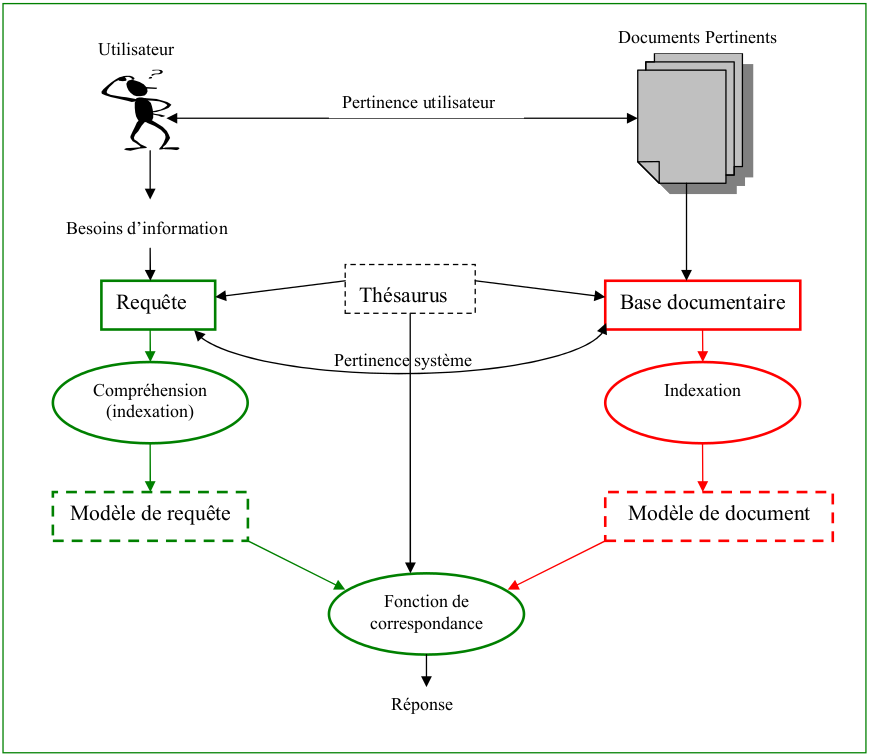
\includegraphics[width=15cm, angle=0]{Figures/Processus-U.png}}
    \end{center}
    \caption{Processus en U de la RI \citep{thesaurus-ir-web}}
    \label{fig:processus-u}
\end{figure}

Pour la suite, on va essayer d’expliquer en détails ce que font chaque partie de ce processus pour mieux élaborer l'étape de la recherche d'information.

\subsection{Première étape: Besoin d'information}
Comme définit dans la section~\ref{sec:besoin-information}, pour qu'une recherche d'information eu lieu, il faudra une besoin d'information. A ce stade la base documentaire est déjà mis en place et est déjà prête pour l'utilisation. L'utilisateur doit ensuite transformer son besoin en requête et obtenir des mots clés. Le système applique un traitement de texte sur la requête pour obtenir une requête finale qui sera utilisé par l'appariement. La requête pourra contenir un ou plusieurs mots clés \citep{modern-ir}.

\begin{definition}[Requête ou Query]
    La requête est une interface entre l'utilisateur et le programme, formulé sous-forme des mots-clés par l'utilisateur décrits en langage naturel \citep{amelioration-ri-approche-semantique}.
\end{definition}

\begin{definition}[Requête ou Query]
    On appelle requête, l'expression du besoin d'information d'un utilisateur. Elle est en général exprimé sous fore des mots clés \citep{salton1989automatique}.
\end{definition}

\subsection{Indexation des documents}
Pour travailler efficacement avec les documents et pour pouvoir rechercher des informations dedans, il faut représenter les documents sous formes des mots clés que contient le document, sous l'approche d'indexation \citep{ir-on-web}.

\begin{definition}
    L'indexation ou tokenisation en anglais est l'action de représenter les contenu des documents sous forme d'index.
\end{definition}

\begin{definition}
    On appelle indexation ou processus d'indexation, le processus qui permet de construire les index a partir de l'analyse du documents tel que la vérification qu'un mot n'est pas dans un anti-dictionnaire (qui n'est pas un mot vide), et la lemmatisation ou racinisation pour trouver la racine des mots. Cette approche est formalisé en utilisant un langage d'indexation. \citep{paradis:tel-00005009}.
\end{definition}

\subsubsection{C'est quoi un index ?}
Un index est est un mot ou groupe des mots sélectionné soit manuellement par un expert, soit automatiquement par un programme informatique (par un ordinateur) pour représenter un document. Les termes d'indexation (index terms) sont tous les index qui représentent un document. Un index est en général un nom ou groupe des noms.

Selon Salton, qui traite généralement les index comme représentant du document, Un index est une représentation synthétique de l'information relative a un document, qui met en évidence sa sémantique en vue d'une requête. Selon d'autres auteurs, se sont des mots clés \citep{paradis:tel-00005009}.

\subsubsection{Approche d'indexation}
Comme on a évoqué précédemment et cité par dans \citep{ir-on-web} ainsi que dans \citep{amelioration-ri-approche-semantique}, il y a en général quatre approche d'indexation tel que l'\textit{indexation manuel}, l'\textit{indexation intelligent}, l’\textit{indexation automatique}, et l'\textit{indexation basé sur les métadonnées}. Il y a une approche \textit{semi-automatique} qui utilise a la fois l'indexation manuelle et automatique (une hybridation), cette approche consiste a créer les index automatiquement puis ces index sont validés par un expert \citep{paradis:tel-00005009}.

\begin{itemize}
    \item[•] \textbf{Indexation manuelle (Human Indexing):} indexation par un humain expert. Cette approche a une avantage d'être plus précise en sélection de terme d'indexation. Tandis qu'avec la croissance de volume d'informations, cette approche est de plus en plus obsolète, ainsi il se peut qu'il y a une incohérence entre les experts en sélectionnant les termes d'indexation. Cette approche est coûteux \citep{evaluation-of-ir-system}.
    \item[•] \textbf{Indexation automatique (Automatic Indexing):} c'est un programme informatique qui fait l'indexation. Cette approche a une avantage d'être moins coûteux qu'un indexation manuel, résout l'incohérence entre les termes d'indexation sélectionné. Mais peut être moins efficace en sélectionnant les index, les index peuvent être moins précise. Cette approche utilise généralement la Traitement de Langage Naturel (NLP) et de la Statistique (Segmentation, Stop words removal).
    \item[•] \textbf{Indexation intelligent (Intelligent Indexing / Agent-Based Indexing):} Utilisation des robots (Spiders / Crawlers) pour l'indexation du WEB. Un robot ou spiders est un programme informatique qui parcours les liens sur le web et index les documents trouées. Cette approche a trois problèmes en général (Robot Standard Exclusion), les robots peuvent causer des surcharge au niveau des serveurs, invasives, et la mise a jour fréquent des sites web.
    \item[•] \textbf{Indexation basé sur les métadonnées:} utilisation et interprétation des métadonnées, souvent utilisé dans la recherche d'information sur le web (HTML).
\end{itemize}

Dans ce document, on focalisera sur l'indexation automatique des documents généralement textuelle (PDF, Document WORD) par un programme informatique.

\subsection{Analyse lexical (Segmentation)}
L'analyse lexical des textes permet de faire une analyse de la lexique. Cette analyse peut varier suivant la langue utilisée. On analyse généralement les ponctuations, les espaces entre les mots et la casse des lettres. On considère que la séparation des mots est le caractère espace. L'analyse lexical est alors l'action de convertir les textes du document en groupe des mots (stream of words) qui peuvent être sélectionné comme termes d'indexation. Les nombres sont souvent une mauvaise index sauf s'il est mixé avec un mot. Les expressions régulières sont souvent utiles pour extraire des nombres comme le numéro de carte de crédit, \dots \citep*{modern-ir, approche-semantique}.

\subsubsection{Ponctuation}
Les ponctuations sont normalement supprimés dans le cas d'analyse lexicales. Sauf dans le cas pour distinguer 'x.id' et 'xid.', la ponctuation ne doit pas être supprimé. \citep{modern-ir}

\subsubsection{Casse des lettres}
Il faut convertir tous les mots en majuscules ou en minuscules. Mais en particulier, les langages de commande (ligne de commande) de Linux, car l'utilisateur ne veut pas convertir la casse des lettres \citep{modern-ir}. Ça peut perdre aussi l'aspect sémantique après la conversation.

\subsection{Élimination des mots vides (Stop words)}
On appelle un mot vide, un mot qui est plus souvent utilisé dans un document ou dans les termes de recherche d'un utilisateur comme les prépositions, les articles, les conjonctions. Certains verbes, adverbes, et adjectifs pouvant être traité comme mots vides. Éliminer ces mots est important car un mot qui apparaît 80\% dans le corpus n'est pas utile pour la recherche d'information. C'est l'action de supprimer les mots insignifiants (pronoms personnels, préposition, \dots) \citep*{modern-ir, approche-semantique, sarch-engine-vsm}.

Voici une liste non exhaustive des mots vides en français selon \citep{stopwords_french}: le, de, du, mais, donc, car, ceci, cela, qui. A noter que pour un SRI Full-text qui prend tous les mots comme des termes d'indexations, il n'y a pas de suppression des mots vides \citep{modern-ir}.

\subsection{Lemmatisation et Stemming}
La lemmatisation ou racinisation de mot est une partie de le traitement de langage naturel (TLN) qui extrait la racine d'un mot pour regrouper les variants (biologiste, biologique -> biologie; suis, est -> être). Cette approche réduit la taille des termes d'indexation \citep*{approche-semantique, sarch-engine-vsm}.

Le Stemming regroupe aussi les variants d'un mot pour obtenir ce qu'on appelle un stem. Un stem est un portion d'un mot restant après la suppression de ses affixes (suffixes, préfixes), la suppression de pluriel, forme gérondif. Cette approche réduit aussi la taille des termes d'indexation. Le stemming ne permet pas de satisfaire la racinisation d'un mot (peut mal déterminer la racine), que certaine moteurs de recherche n'adopte pas le stemming \citep*{modern-ir, vsm}.

Le stemming possède plusieurs techniques, mais on va citer les techniques principaux qui sont:

\begin{itemize}
    \item[•] \textbf{Table lookup}: regarder le stem dans un table, mais qui est moins pratique en terme de stockage et accessibilité.
    \item[•] \textbf{Porter algorithme}: est une technique simple, intuitive, peut être implémenté efficacement. Cette approche utilise la suppression des affixes.
    \item[•] \textbf{Successeur}: est un approche plus complexe que la suppression des affixes.Se base utilisation des connaissances linguistiques structurés pour identifier les morphes.
    \item[•] \textbf{N-Grams}: est une approche orienté plus vers la classification que stemming. Cette approche se base sur l'identification des diagrammes et trigrammes.
\end{itemize}

D'autres méthodes sont disponibles actuellement comme celle qui se base sur les expressions régulières, \dots

\subsection{Normalisation}
La normalisation permet de classer les termes comme équivalent. Par exemple, le mot U.S.A doit être traité de la même façon que USA. Cette approche de normalisation peut amener a des problèmes \citep{sarch-engine-vsm}.

\subsection{Sélection et pondération des termes}
Comme on dit précédemment, pas tous les mots dans le documents sont significatifs. Sauf pour un moteur de recherche full-text qui index tous les termes. Et aussi pas tous les mots on une même degré ou poids d'importance dans un document. D'où la pondération des termes. Pour déterminer le poids d'un terme dans un collection des documents, on utilise en général deux approche: \textit{Term Frequency (TF)} et \textit{Inverse Document Frequency (IDF)}.

\textit{Le TF (Term Frequency)} du terme \textit{t} dans un document \textit{d} est le nombre de fois où le terme t apparaît dans le document d. C'est la fréquence du ter t dans le document d. Plus ce fréquence est important, plus le terme est important pour représenter le document. Cette mesure sera normalisé afin d'éviter d'avoir un poids trop significatifs pour les documents avec beaucoup de contenu, on l'appelle \textit{Normalized Term Frequency}.

\textit{L'IDF (Inverse Document Frequency)} du terme t dans la collection des documents D est le nombre de document dans la collection contenant le terme t. C'est le nombre de document où le terme t apparaît dans la collection des documents D. Cette approche permet de déterminer l'unicité d'un terme au sein de la collection des documents. Un terme est important si moins de documents la contiennent; un terme qui apparaît dans presque tous les documents n'est pas significatif, et peut être traité comme un mot vide.

La troisième approche qui est la combinaison des deux est la \textit{TF-IDF}. La TF-IDF est la multiplication des deux valeurs obtenues précédemment ($TF*IDF$) pour obtenir le poids final du terme. Le terme est important s'il apparaît dans peu de documents (IDF) mais qu'il apparaît plusieurs fois dans le document qui le contient (TF).

Une fois ces termes sélectionné avec les poids correspondant, on crée un index inversé ou fichier inversé pour stocker ces termes. Cet index inversé va faire correspondre le document identifié par un ID avec les termes qui le compose avec le poids correspondant \citep*{vsm, vsm-for-arabic-language, sarch-engine-vsm, modern-ir}. Tous ces notions va être détaillé un peu plus bas dans le document lorsqu'on abordera le modèle utilisé dans le cadre de ce mémoire.

\subsection{Étape d’appariement}
\label{sec:etape-appariement}
Pour pouvoir satisfaire le besoin de l'utilisateur, il faut apparier la requête de l'utilisateur et les documents (fichier inversé) en utilisant un algorithme d'appariement. Ces algorithmes permet de calculer la similarité entre un document et une requête et savoir 
quels sont les documents qui correspondent le mieux avec la requête avec un degré de similarité. Mathématiquement, c'est calculer la distance euclidien entre la requête et le document.

On calcule ces mesures pour déterminer la pertinence entre la requête de l'utilisateur et les documents dans le corpus, on l'appelle \textit{pertinence système}. Il y a aussi le jugement qui provient de l'utilisateur en vue des résultats qu'il obtient par rapport a sa demande, on l'appelle \textit{pertinence utilisateur} \citep{vsm-images}.

La notion de pertinence est très complexe. En général un document est pertinent si l'utilisateur trouve les informations qui satisfait ses besoins dans le document. C'est sur ce notion de pertinence que le SRI doit juger la pertinence. \citep{salton1989automatique}

Les documents trouvés sont retournés a l’utilisateur généralement suivant un degré de pertinence décroissante par rapport a la requête. Certains modèle ne possède pas ce classement des résultats comme le modèle Booléen qu'on va voir dans la section précédente, ainsi que décortiquer ces mesures de similarité.

\subsection{Reformulation de la requête}
La requête de l'utilisateur est parfois courte ou incomplète, alors il faut reformuler la requête par l'ajoute, modification ou suppression des mots clés dans la requête. Il est aussi possible de modifier le poids des termes dans la requête. Parmi les différentes approches proposé, \citeauthor{amelioration-ri-approche-semantique} \citep{amelioration-ri-approche-semantique} note trois approches utilisé dans la reformulation de la requête tel que:

\begin{itemize}
    \item \textbf{Thésaurus}: cette approche utilise une base de connaissance linguistiques pour améliorer la requête de l’utilisateur.
    \item \textbf{Basé sur les co-occurrences}: utilisent le calcul basé sur des co-occurrences des termes.
    \item \textbf{Relevance feed-back}: cette approche se base sur la reformulation de la requête par l'utilisateur par rapport aux pertinences des documents qu'ils reçoivent. En rajoutant, modifiant ou enlevant des termes de recherche ou mots clés.
\end{itemize}

\section{Modèle de RI}
\subsection{Introduction}
Il y a deux raisons pour avoir un modèle dans la recherche d'information. La première, un modèle guide la recherche et donne sens a la discussion académique. La seconde, un modèle sert comme un plan (blueprint) modèle pour implémenter un système de recherche d'information \citep{model-ir}.

Un modèle sert a décrire le processus computationnel du RI (comment les documents sont stockés, comment sont stocké les index, etc.), décrire le processus humain (besoin d'information, interaction), ainsi la définition implicite ou explicite de la pertinence \citep{model-ri-cours}.

Pour bien formaliser la recherche d'information, il est nécessaire de définir des modèles a utiliser. L'étape d’appariement dans la section Étape d'appariement, nécessite un modèle.

\subsection{Caractéristique formel (DQFR)}
\begin{definition}
    Un modèle de recherche d'information est quadruplet DQFR tel que \citep*{modern-ir, vsm}:
    \begin{itemize}
        \item \textbf{D}: ensemble des représentation (vue logiques) des documents dans la collection
        \item \textbf{Q}: ensemble des représentation (vue logiques) des besoins de l'utilisateur. On l'appelle requête ou query en anglais.
        \item \textbf{F}: framework pour modéliser les documents, la requête ainsi que leurs relations.
        \item \textbf{R $(q_{i}, d_{j})$}: fonction de classement qui associe un nombre réel avec la requête qi appartient a \textit{Q} et le document $d_{i}$ appartient a \textit{D}. Cette classement permet d'ordonner les résultats selon leur pertinence.
    \end{itemize}
\end{definition}

\subsection{Taxonomie de modèle}
Selon \citeauthor{modern-ir} il y a quatre familles principales des modèles de RI qui est illustré dans la Figure~\ref{fig:modele-ri}:

\begin{itemize}
    \item \textbf{Les modèles basé sur les textes du document}: les modèles de RI classique (\textit{Théorie des ensembles, Algébrique, Probabiliste}), et les modèles basé sur le texte semi-structuré (\textit{Texte semi-structuré})
    \item \textbf{Les modèles basé sur le liens entre documents}: les modèles orienté web (\textit{PageRank, Hubs et autorités})
    \item \textbf{Les modèles basé sur les documents multimédia}: les modèles de recherche d'images, vidéos, musiques, etc.
\end{itemize}

\begin{figure}[htbp]
    \begin{center}
        \fbox{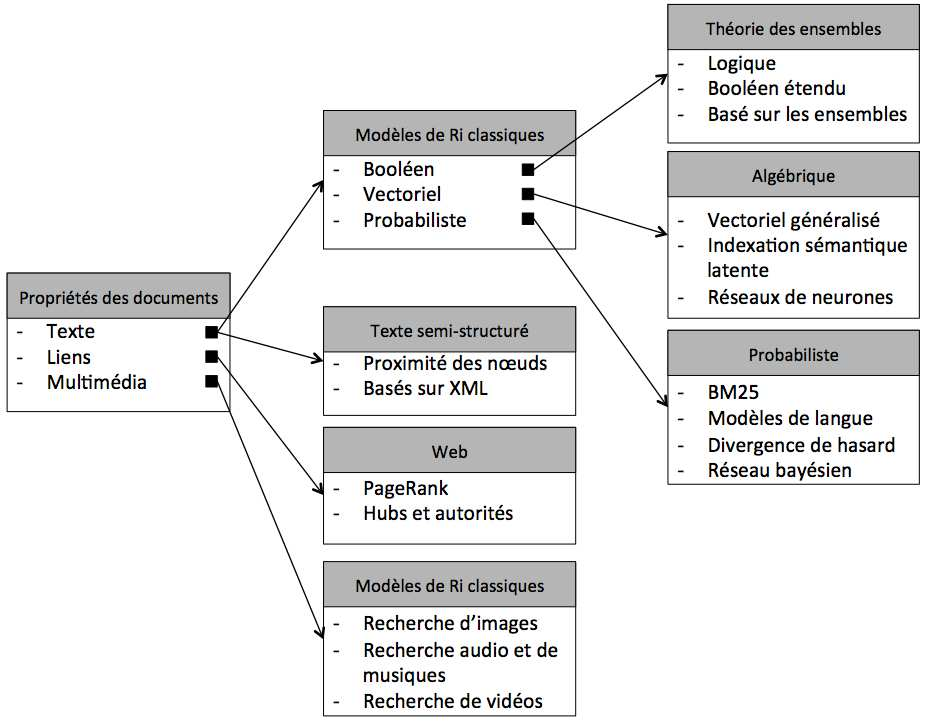
\includegraphics[width=15cm, angle=0]{Figures/modele-ri.png}}
    \end{center}
    \caption{Taxonomie de modèle de RI \citep{soulier2014:def-evaluation-modele}}
    \label{fig:modele-ri}
\end{figure}

Dans le cadre de ce mémoire, on va analyser la famille des modèles classiques basé sur les textes du document, car ce qui concerne mieux notre étude.

\subsection{Catégorie de modèle}
Comme énoncé précédemment, on va s’intéresser dans la famille des modèles classiques basé sur les textes du document. Dans cette famille, on a \citep*{modern-ir, approche-semantique,soulier2014:def-evaluation-modele}, il y a trois grandes catégories des modèles: le modèle \textbf{théorique ou ensembliste} (theoretic), le modèle \textbf{algébrique} (algrebraic) et le modèle \textbf{probabiliste} (probabilistic).

Dans le modèle ensembliste, on trouve principalement le modèle \textbf{Booléen}, le modèle \textbf{Booléen étendue}. Dans le modèle algébrique, on a principalement le modèle \textbf{vectoriel} (Vector Space Model), le modèle de \textbf{réseau de neurone} (Neural Network Models), et d'autres modèles. Dans le modèle probabiliste, on trouve principalement le modèle probabiliste (Probabilistic model), le \textbf{réseau d'inférence} (Inference Network) et d'autres modèles.

Ces modèles sont des modèles de recherche, mais il y a aussi des modèles pour la navigation (Browsing). Pour plus de détails \citep{modern-ir}.

\subsection{Modèle ensembliste}
Dans le modèle ensembliste, il y a quelques modèles, mais dans le cadre de ce mémoire, on va voir les deux principaux.

\subsubsection{Modèle Booléen (Boolean Model)}
Un exemple de requête dans le modèle Booléen est illustré sur la Figure~\ref{fig:boolean-model}.

\begin{figure}[htbp]
    \begin{center}
        \fbox{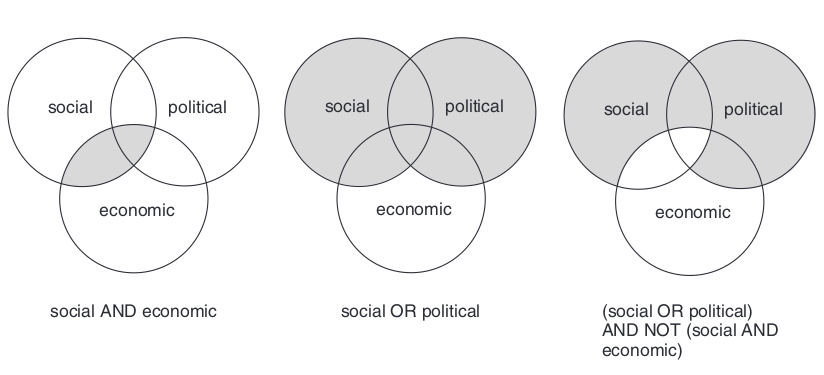
\includegraphics[width=15cm, angle=0]{Figures/boolean-model-example.png}}
    \end{center}
    \caption{Exemple de diagramme de requête de modèle Booléen \citep{model-ir}}
    \label{fig:boolean-model}
\end{figure}

Ce un modèle de base dans la recherche d'information. Ce modèle est le premier modèle utilisé dans la recherche d'information. Dans ce modèle, les documents et les requêtes sont représentés comme des mots clés (ensemble des mots). Ce modèle est simple, facile a mettre en place et utilise l'algèbre de Boole. La stratégie de recherche est basé sur la décision binaire.
Ce modèle a possède un avantage d'être facile a mettre en place, simple et exacte au niveau des résultats. Ce pour cette exactitude que ce modèle est aussi un modèle exacte (Exact Match Model).

Les termes sont pondérés de façon binaire.

Tous les termes d'indexation ont la même poids, soit il existe dans le document soit non. S'il existe dans le document, son poids est 1, sinon 0. La similarité entre $q$ et $d_{j}$ est égal a 1 si le document terme $d_{j}$ valide l'expression booléen $q$, sinon 0. Un document est donc jugé pertinent par le système s'il valide l'expression booléen de la requête.

Dans ce modèle, la requête est exprimé en utilisant les opérateurs booléens ET (AND), OU (OR) et NON (NOT).

Par contre, ce modèle a quelques inconvénients, il est difficile de transformer la besoin d'information en expressions booléen surtout pour un utilisateur lambda (un utilisateur qui ne sait absolument rien de l'expression booléen) donc la requête a tendance un peu simplifié ou même incomplète ce qui affecte la qualité des résultats. Et puisque la décision est binaire, et que le poids soit 1 soit 0, il n'y a pas de classement possible pour les documents retournés. L'utilisateur est alors obligé de parcourir les résultats pour juger la pertinence. Puisque le modèle est exacte, le modèle ne permet pas de sélectionner les documents qui peuvent intéressé l'utilisateur et qui peuvent être pertinent par rapport a ses requête, et qu'il est impossible de récupérer une réponses partielles qui valide certains expression de la requête. \citep*{modern-ir, soulier2014:def-evaluation-modele}.

\begin{definition}[Modèle booléen]
    On note $w_{ij} \in \{0, 1\}$ le poids du terme numéro $i$ dans le document numéro $j$ qui est binaire $ \vec{q}_{dnf} $, forme normal de disjonction de la requête $ q $. Considérons $ \vec{q}_{cc} $ composant conjonctive de $ \vec{q}_{dnf} $. La similarité du document $ d_{j} $ par rapport a la requête $ q $ est définie par:

    \[
        Sim(d_{j}, q) = \left\{
        \begin{array}{ll}
            0 & Sinon \\
            1 & \textit{S'il } \exists \vec{q}_{cc} \mid (\vec{q}_{cc} \in \vec{q}_{dnf}) \bigwedge (\forall k_{i}, g(\vec{d_{j}}) = g_{i}(\vec{q}_{cc}))
        \end{array}
        \right.
    \]

    Si $ Sim(d_{j}, q) = 1$, le document $ d_{j} $ est pertinent a la requête $ q $; dans le cas contraire, le document n'est pas pertinent par rapport a la requête.
\end{definition}

\subsubsection{Modèle Booléen Étendu (Extended Boolean Model)}
En vue de ces inconvénients, le modèle booléen est amélioré afin de résoudre certains problèmes avec le modèle Booléen. Premièrement, le modèle Booléen étendue a mis en place la possibilité de faire une similarité partiel et la pondération des termes. Il est étendu en ajoutant la fonctionnalité du modèle vectoriel qui est la combinaison de formulation de requête avec les caractéristiques du modèle vectoriel. Ce modèle est introduit par Salton, Fox, et Wu en 1983. Mais ce modèle n'a pas été largement utilisé \citep{modern-ir}.

\subsubsection{D'autres modèles}
Il y a aussi d'autres modèles dans la catégorie ensembliste, tel que le modèle de Fuzzy (Fuzzy Set Model, Region Models), \dots, mais qui ne sont pas détaillé dans le cadre de ce mémoire. Pour plus de détails, voir chapitre 2 \citep{modern-ir} et chapitre 1 \citep{model-ir}.

\subsection{Modèle algébrique}
Dans cette catégorie, on va analyser le modèle vectoriel principal.

\subsubsection{Modèle Vectoriel (Vector Space Model)}
\label{sec:vsm-model}

Ce modèle a un alternative qui est le Modèle Vectoriel Généralisé par Salton \citep{salton1975vector}, qui se base sur des vecteurs. Les documents et les requêtes sont représentés par un vecteur dans un t-espace vectoriel (représentation algébrique). Ce modèle accorde une appariement partielle, et les termes ne sont pas pondérés de manières binaires. Les pondérations des termes le plus souvent utilisé sont la TF, IDF, et la TF-IDF \citep*{sarch-engine-vsm}.

Un score de similarité est alors exprimé comme un mesure de proximité entre deux entités correspondant a l'angle qui sépare les deux vecteurs. On va analyser brièvement ces mesures dans la section \ref{sec:mesure-similarite}.

\begin{figure}[htbp]
    \begin{center}
        \fbox{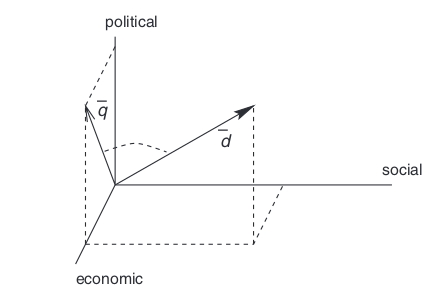
\includegraphics[width=10cm, angle=0]{Figures/vector-model.png}}
    \end{center}
    \caption{Représentation du document et la requête dans le modèle vectoriel \citep{model-ir}}
    \label{fig:vector-model}
\end{figure}

Le modèle vectoriel a certains avantages: Facile a mettre en œuvre, possibilité d'avoir un appariement approximatif avec un degré de pertinence (L'utilisateur reçoit des documents qui pourrait lui intéressé), possibilité d'organiser les résultats suivant leur pertinence (L'utilisateur passe moins de temps a filtrer les résultats puisqu'ils sont déjà ordonné), ainsi ce modèle peut définir une limité pour la mesure de similarité et de n'afficher que les documents qui sont en dessus de cette limite pour éliminer les résultats le moins pertinent. Ce modèle est populaire, et plus utilisé par les moteurs de recherche actuel. \citep*{approche-semantique, modern-ir, soulier2014:def-evaluation-modele}

Mais ce modèle a un inconvénients, qui est l’indépendance des termes d'indexation ce qui implique que la notion de sémantique du document est perdue. Mais ce problème a été solutionné par la mise place de regroupement des termes qui ont la même sens, on appelle N-grammes. Ou bien une autre approche est d'utiliser le modèle d’indexation sémantique latente (Latent Semantic Index).

\begin{definition}[Modèle Véctoriel]
    On note $w_{ij}$ le poids positif et non binaire, du terme i dans le document j qui est associé avec un pair $(k_{i}, d_{j})$ et $w_{iq}$ le poids du terme i dans la requête $q$. La requête est définie par le vecteur: $ \vec{q} = (w_{1q}, w_{2q}, \dots, w_{tq}) $ où $t$ le nombre total des termes d'indexation dans le système. Un document $d_{j}$ est présenté par le vecteur: $ \vec{d_{j}} = (w_{1j}, w_{2j}, \dots, w_{tj}) $.

    La calcul de similarité entre ces deux vecteurs se traduit par la formule:
    \[
        Sim(\vec{d}, \vec{q}) = \frac{\vec{d_{j}} \cdot \vec{q}}{ |\vec{d_{j}}| \times |\vec{q}| } \\
        = \frac{\sum_{i=1}^{t} w_{i,j} \times w_{i,q}}{\sqrt{\sum_{i=1}^{t} (w_{i,j})^2} \times \sqrt{\sum_{i=1}^{t} (w_{i,q})^2}}
    \]

    Avec $ |\vec{d_{j}}| $ et $ |\vec{q}| $ norme du vecteur document et de la vecteur requête.
\end{definition}

\subsubsection{Autre modèle}
Il y a d'autres modèles dans la catégorie algébrique tel que le modèle d'Indexation Sémantique Latente (Latent Semantic Indexing) et le modèle de réseau de neurones (Neural Network Model).

L'approche d'indexation sémantique latente est introduit en 1988, qui permet de garder la sémantique des documents pour avoir une relation entre les termes d'indexation. Cette approche se base sur l’appariement de contexte au lieu d'index, voir \citetitle[Page 45]{modern-ir} \citep{modern-ir} pour les détails complet.

Le modèle neuronale se base sur des processus d'activation des neurones (spread activation process), cette approche est plus orienté vers l’intelligence artificielle \citep*{modern-ir}.

\subsection{Modèle probabiliste}
Dans le modèle probabiliste, le framework pour modéliser les documents et la représentation de la requête se base sur la théorie des probabilités. On va pas rentrer dans les détails sur ce modèle, mais juste un tour d'horizon. Pour ce qui veulent entrée dans les détails, voir chapitre 2 de \citep{modern-ir}.

\subsubsection{Modèle probabiliste}
\begin{figure}[htbp]
    \begin{center}
        \fbox{
\includegraphics[width=15cm, angle=0]{Figures/probabilistic-model.png}}
    \end{center}
    \caption{Diagramme de collection pour le terme social dans le modèle probabiliste \citep{model-ir}}
    \label{fig:probabilistic-model}
\end{figure}

Le principe du modèle probabiliste est de donner la requête $q$ de l'utilisateur et un document $d_{j}$ dans la collection. Puis le modèle estime la probabilité que l'utilisateur trouve le document $d_{j}$ pertinent. Le modèle assume que ce probabilité de pertinence dépends seulement de la requête et la représentation du document. La mesure de similarité utilise la formule de Bayes (Bayes's rule). Pour plus de détails voir Section 1.4 \citep{model-ir} ou chapitre 2 \citep{modern-ir}.

\begin{definition}[Modèle probabiliste]
    On note $w_{ij} \in \{0, 1\}$ le poids du terme $i$ dans le document $j$, et $w_{iq} \in \{0, 1\}$ le poids du terme $i$ dans la requête $q$.\\
    $R$: Ensemble des documents connu ou initialement estimé d'être pertinent.\\
    $\bar{R}$: Complément de $R$, l'ensemble de documents non pertinent.\\
    $P(R/d_{j})$: Probabilité de pertinence du document $d_{j}$ pour la requête $q$. \\
    $P(\bar{R}/d_{j})$: Probabilité de non pertinence du document $d_{j}$ pour la requête $q$.

    \[
        Sim(d_{j}, q) = \frac{ P(R/\vec{d_{j}}) }{ P(\bar{R}/\vec{d_{j}}) } = \frac{P(\vec{d_{j}}/R) \times P(R)}{P(\vec{d_{j}}/\bar{R}) \times P(\bar{R})}
    \]

    Où:\\
    $ P(d_{j}/R) $: Probabilité de sélection du document $ d_{j} $ au hasard provenant de l'ensemble $ R $ des documents pertinents.\\
    $ P(R) $: Probabilité qu'un document sélectionné au hasard dans la collection entière est pertinent.

    Or, $ P(R) $ et $ P(\bar{R}) $ est la même pour tous les documents, alors la formule de similarité devient:
    
    \[
        Sim(d_{j}, q) \sim \frac{P(\vec{d_{j}}/R)}{P(\vec{d_{j}}/\bar{R})}
    \]

    Avec l'application des poids de terme, la formule de similarité final est donc:
    \[
        Sim(d_{j}, q) \sim \sum_{i = 1}^{t} (w_{iq} \times w_{ij}) \times \left(
            \log{\frac{P(k_{i}/R)}{1 - P(k_{i}/R)}} + \log{\frac{P(k_{i}/\bar{R})}{1 - P(k_{i}/\bar{R})}}
        \right)
    \]

    Tel qu'au départ:\\
    $ P(k_{i}/R) $: $ 0.5 $ \\
    $ P(k_{i}/R) = \frac{n_{i}}{N} $ avec $ n_{i} $ le nombre de documents qui contient le terme $ k_{i} $, et $ N $ le nombre total des documents.
\end{definition}

Ce modèle a un avantage d'avoir le classement des résultats suivant leur probabilité d'être pertinent dans l'ordre décroisant. Mais a quelques inconvénients qui est le besoin de savoir initialement la séparation des documents en ensembles pertinent et non pertinent, le modèle ne prend pas en compte le fréquence de terme dans un document ce qui implique que tous les poids des termes sont binaire, ainsi les termes d'indexation sont indépendants \citep{modern-ir}.

\subsubsection{Autres modèles}
Il y a d'autres modèles dans ce catégorie, mais comme tous les autres on va pas rentrer dans les détails puisque ça va a l’encontre de notre analyse. On cite le Réseau d'Inférence (Inference Network), Réseau Bayésien (Bayesian Network), le modèle de Poisson (The 2-Poisson model) \citep{model-ir}. Pour plus de détails voir \citep{modern-ir}.

\section{Mesure de similarité}
\label{sec:mesure-similarite}
Citons quelques méthode de similarité \citep*{vsm-for-arabic-language, sarch-engine-vsm, vsm}:
\begin{itemize}
    \item[•] \textbf{Produit scalaire (Dot Product)}: c'est le produit scalaire entre deux vecteurs. La requête et les documents sont représenté par des vecteurs de même dimension.
    \item[•] \textbf{Similarité cosinus (Cosine Similarity)}: c'est la mesure le plus populaire. Utilise le produit scalaire ainsi que l'angle formé entre les deux vecteurs (document et requête)
    \item[•] \textbf{Coefficient de Jaccard (Jaccard Coefficient)}: mesure statistique de similarité entre des collections (sample set)
    \item[•] \textbf{Coefficient de Dice (Dice Coefficient)}: même que celle de Jaccard, mais double le poids de vecteur
\end{itemize}

Puisque nous-nous intéressons au modèle vectoriel dans le cadre de ce mémoire, on va analyser les mesures de similarité utilisé dans ce modèle. Il y a principalement quatre mesures de similarité comme on a présenté dans la section \ref{sec:etape-appariement}. Ces mesures sont utilisé pour déterminer la pertinence système c'est a dire la pertinence des documents par rapport a la requête de l'utilisateur. A bien noter que tous les poids des termes d'indexation sont normalisé avec TF-IDF avant la calcul de ces mesures. Ces mesures sont optionnelles, mais la mesure de similarité le plus populaire est celle de Cosinus \citep{vsm}.

La pondération des termes se traduit alors comme suit:
\[
    d_{k} = q_{k} = tf(k, d) \cdot \log{\frac{N}{df{(k)}}}
\]

Avec:
Term Frequency (TF):
\[
    TF(t, d) = \frac{\textit{Nombre d'occurences du terme} t \textit{ dans le document } d}{\textit{Nombre total des termes dans le document } d}
\]

Inverse Document Frequency (IDF):
\[
    IDF(t, D) = \log\frac{\textit{Nombre total des documents dans le corpus } N}{\textit{Nombre de documents qui contient le terme } t}
\]

Term Frequency-Inverse Document Frequency (TF-IDF):
\[
    TF-IDF(t, d, D) = \textit{TF}(t, d) \times \textit{IDF}(t, D)
\]

\subsection{Produit scalaire}
Le produit scalaire ou Dot product (Inner Product) en anglais est la mesure de base, qui est utilisé dans d'autres mesure comme celle de cosinus, Jaccard ainsi que Dice. Cette mesure calcul le produit scalaire entre le vecteur document et la vecteur requête. La formule pour calculer ce mesure est ci-dessous:

\[
    Inner Product(\mathbf{A}, \mathbf{B}) = \mathbf{A} \cdot \mathbf{B}
\]

\subsection{Similarité cosinus}
La mesure cosinus ou Cosine Similarity est la mesure la plus populaire. Cette mesure utilise le produit scalaire en introduisant l'angle formé par les deux vecteur (document et requête). La formule pour calculer cette mesure est ci-dessous:

\[
    Sim(\vec{d}, \vec{q}) = \frac{\vec{d} \cdot \vec{q}}{\|\vec{d}\| \cdot \|\vec{q}\|} = \frac{\sum_{k=1}^{n} d_{k} \cdot q_{k}}{\sqrt{\sum_{k=1}^{n} (d_{k})^2} \cdot \sqrt{\sum_{k=1}^{n} (q_{k})^2}}
\]

\subsection{Similarité de Jaccard}
La mesure de Jaccard ou Jaccard's Similarity utilise aussi le produit scalaire, c'est une mesure basé sur la statistique. La formule pour calculer cette mesure est ci-dessous:

\[
    \textit{Jaccard Similarity}(A, B) = \frac{|A \cap B|}{|A \cup B|}
\]

\subsection{Similarité de Dice}
La mesure de Dice ou Dice's Similarity est la mesure utilise le produit scalaire. La formule pour calculer cette mesure est ci-dessous:

\[
    \textit{Dice Similarity}(A, B) = \frac{2 |A \cap B|}{|A| + |B|}
\]

\section{Conclusion}
En guise de conclusion de cette partie qui concerne la recherche d'information, qu'il y a beaucoup des chercheurs qui s'y intéressent puisque c'est un domaine vaste, intéressant mais aussi difficile et possède des défis. C'est un domaine ancien mais qui a connu des évolutions considérable jusqu’à nos jours avec l'explosion de volume d'information disponible sur internet par le biais des réseau sociaux, des blogs, etc. On a vue dans cette partie qu'il y a des modèles mathématique appliqués dans ce modèle ce qui rend la recherche formalisé. Ainsi l'amélioration de ces modèles par le biais de l’intelligence artificielle est possible, ce qui est le cas des géants des moteurs de recherche modernes aujourd'hui.

On a vue dans cette partie qu'il y a beaucoup des modèles utilisés dans la RI, des mesures et d'algorithme de calcul de similarité ainsi que de classement des résultats.

Analysons de plus près dans la section suivante ce qui concerne le Système de Recherche d'Information (moteur de recherche).